\chapter{ผลการพัฒนา}
\label{chapter:result}

ทีม Manyfox มีการประเมินผลการพัฒนาโดยการวัดผลจาก 2 ด้านคือ เชิงประสิทธิภาพ และ เชิงประสิทธิผล
โดยมีวิธีการในการประเมินผลการพัฒนาดังนี้

\section{การประเมินผลเชิงประสิทธิภาพ}
การประเมินผลเชิงประสิทธิภาพใช้ เว็บไซต์ \textbf{https://web.dev} ที่เป็นเครื่องมือของ google ในการประเมินผลออกมาเป็นตัวเลข และแสดงถึงจุดบกพร่อง 
โดยแยกออกมาเป็น 4 ด้านดังนี้
\begin{figure}[!htbp]
	\centering
	
\includegraphics[width=0.8\linewidth]{webdev-logo}
	\caption{Web.dev logo}
	\label{Fig:wed-dev}
\end{figure}
\subsection{Performance}
ประเมินผลจากการตรวจสอบระยะเวลาการโหลดหน้าแรก (ส่วนที่มองเห็นครั้งแรกเมื่อเปิดหน้าเว็บไซต์)
\subsection{Accessibility}
ตรวจสอบปัญหาทั่วไปที่อาจมีผลถึงการะเข้าถึงเนื้อหาบทความ
\subsection{Best practices}
ตรวจสอบรูปแบบโค้ดทั้งหมด ที่ควรเขียนในแบบที่ควรเป็น
\subsection{SEO}
ตรวจสอบ Best practices เฉพาะในส่วน SEO เพื่อให้มั่นใจว่าสามารถค้นหาผ่านทาง Google search เจอ
\newpage
\begin{figure}[!htbp]
	\centering
	\subfigure[ผลการประเมิน Manyfox Web Appication]{
		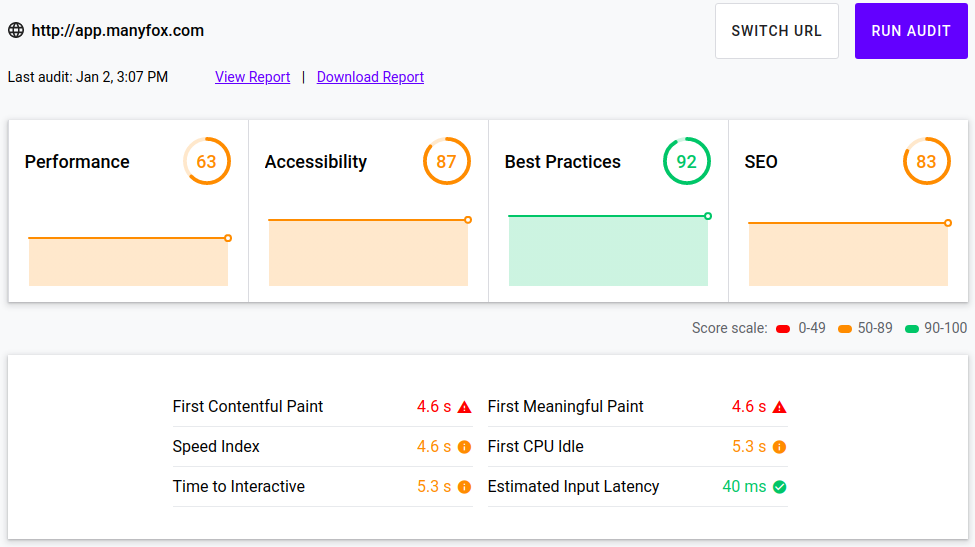
\includegraphics[width=1\linewidth]{audit-app}
		\label{Fig:audit-app}
	}
	\subfigure[ผลการะประเมิน Manyfox Web Landing page]{
		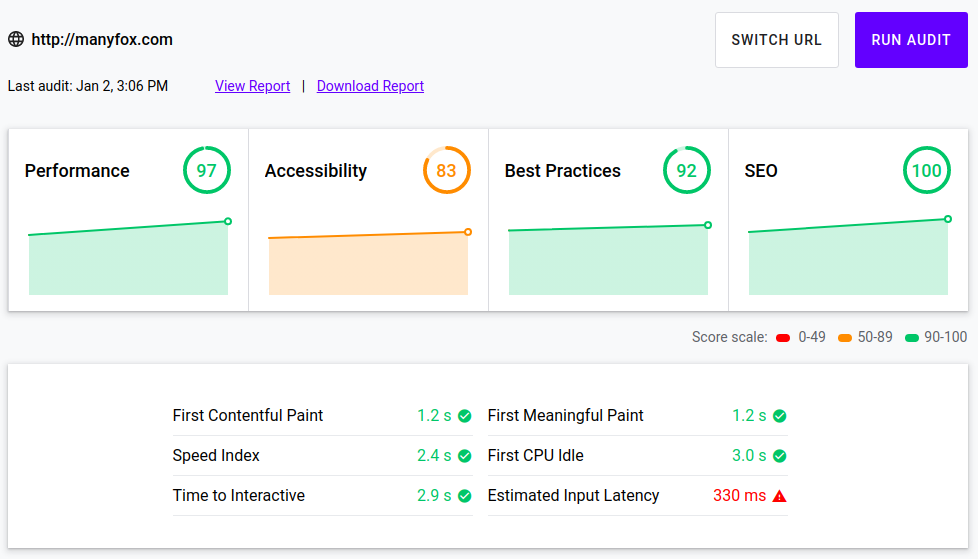
\includegraphics[width=1\linewidth]{audit-landing-page}
		\label{Fig:audit-landing-page}
	}
	\caption{ผลการประเมิน Manyfox}

\end{figure}

\section{การประเมินผลเชิงประสิทธิผล}
การประเมินผลเชิงประสิทธิผลโดยวัดจากความพึงพอใจของผู้ใช้ เพื่อให้เข้าถึงการรับฟังความเห็นจากผู้ใช้ได้มากขึ้น จึงพัฒนา Feedback page
เพื่อรับฟังความเห็น หรือปัญหาจากผู้ใช้